\section{Prediction of cell organelles}
\subsection{Overfitting}

\begin{definition}[Overfitting]
    "Hypothesis overfits the training samples if some other hypothesis that fits the training samples less well actually performs better over the entire distribution of instances" (p67 Mitchell Machine Learning 1997).
\end{definition}

Overfiting prevents model to generalize well on the unseen data and in order to avoid fitting to closely to the training dataset one has several options:

\begin{figure}[htb]
	\begin{center}
		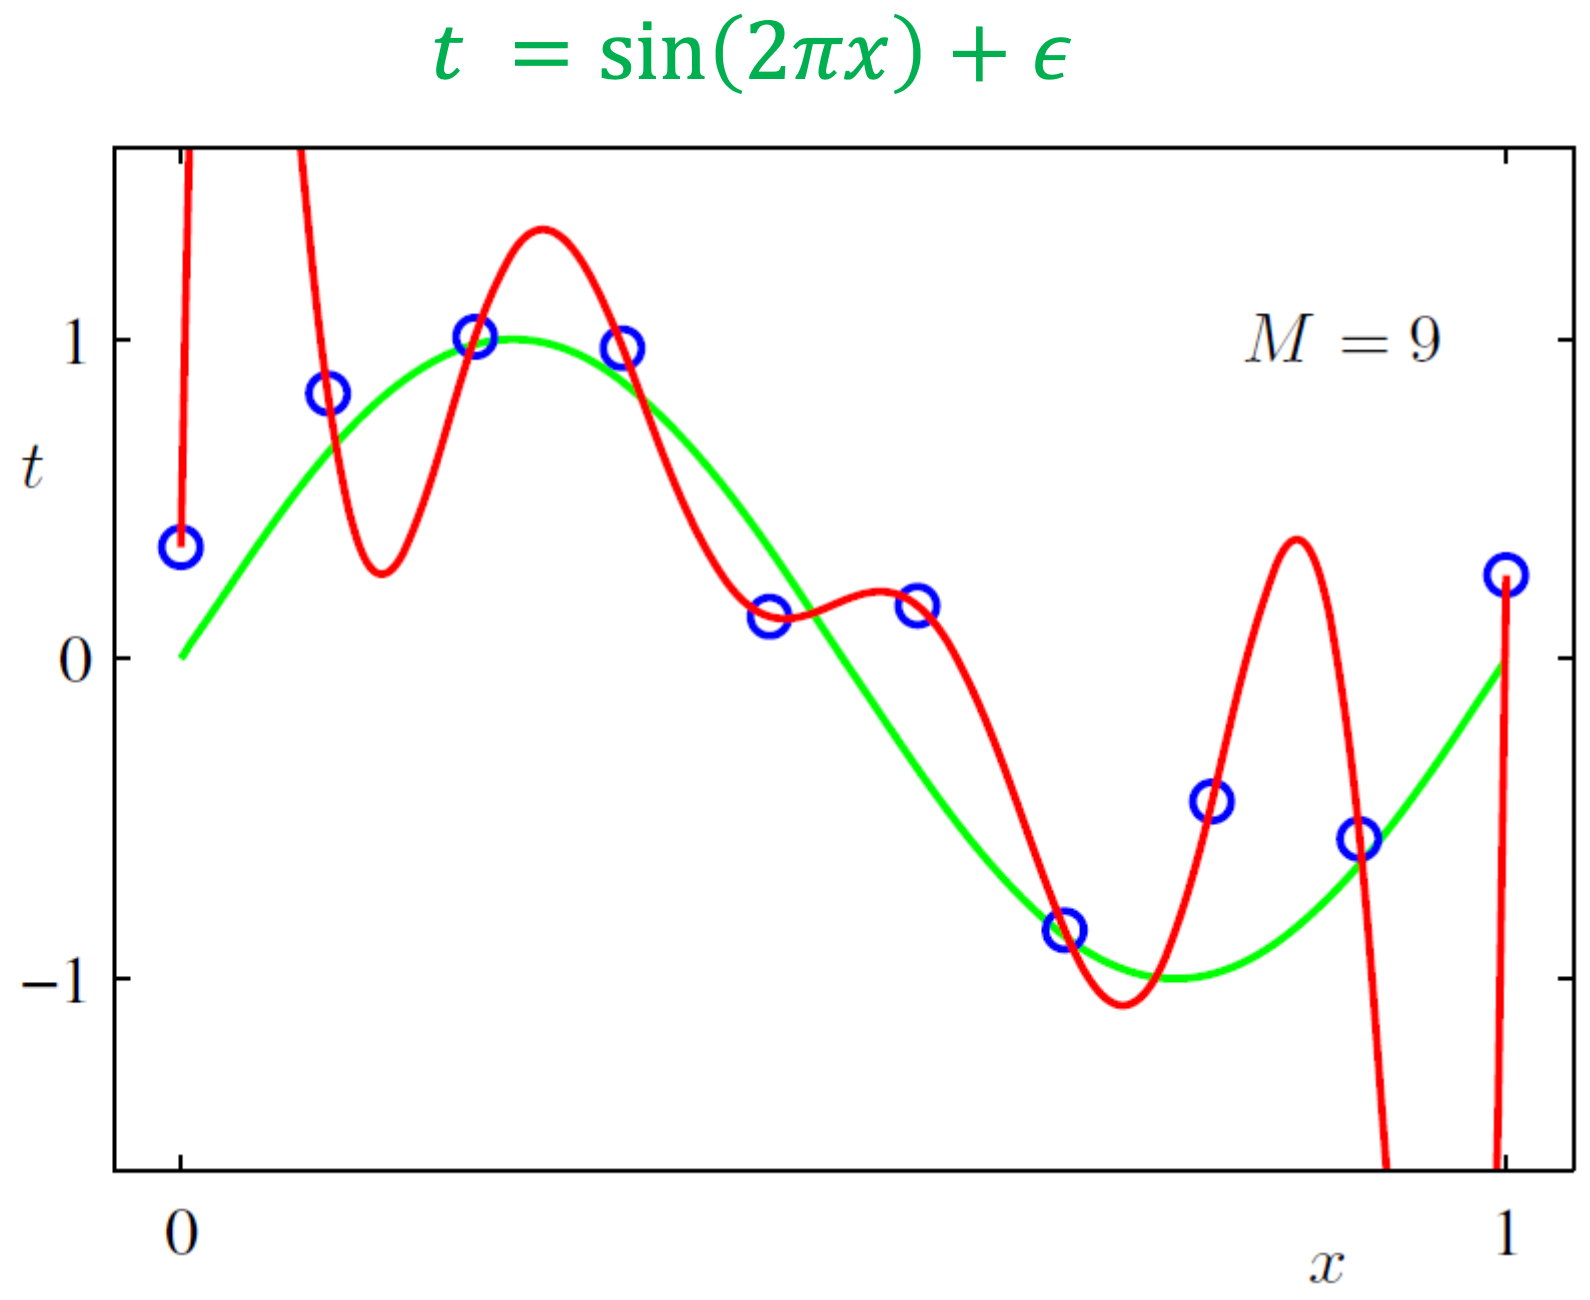
\includegraphics[width=0.6\linewidth]{bilder/overfit.png}
		\caption{Overfitting}\label{fig:overfit}
	\end{center}
\end{figure}

(Bishop book)

\subsubsection{Early-stopping}
Overfitting effect occurs at later epochs. This doesn't happen during early epochs as with the correct weights initialization the weights of the model are quite small and random and therefore the best decision surface would be a smooth one. But in the later epochs the difference in values of the weights grows and they become not similar anymore which means also that the decision surface becomes more complex and will be ble to fit not only the training data itself, but also its noise. (p111 Mitchell Machine Learning 1997). And that is why stopping before the model became too complex for the given data may mitigate this problem.

\subsubsection{Regularization}

The complexity of the model grows with the number of features it uses, sometimes the model may pay attention to the features that are not important to the outcome, or even considers a noise to be a feature. To prevent this one should decrease the weights associated with useless features, however we cannot know ahead which of them should be ignored, therefore one may limit them all. (doi:10.1088/1742-6596/1168/2/022022) In order to do that, a penalty term in loss function is added:

\begin{equation}
   \tilde{L}(\theta, X, y) = L(\theta, X, y) + \lambda R(\theta)
\end{equation}

for some $\lambda > 0$. This is called a \emph{soft-constrait} optimization. When $R(\theta)$ is of the form $R(\theta) = ||\theta||^2_2 = \sqrt{\sum_i \theta_i^2}$ this is called \emph{L2-regularization} and when it is of form $R(\theta) = |\theta||_1 = \sum_i |\theta_i|$ this is called \emph{L1-regularization}. \emph{L2-regularization} used in combination with backpropagation is equivalent to weight decay. Weight decay is defined by Hanson and Pratt (1988) as follows:
\begin{equation}
    \theta_{t+1} = (1 - \lambda)\theta_t - \alpha \frac{\partial L}{\partial \theta_t}
\end{equation}

where $\alpha$ is a learning rate. Weight decay successfully affects more those weights the gradient change along which is smaller (Goodfellow Deep learning p229). \emph{L1-regularization} induces sparsity of the weights by assining some of them to zero, this could be also considered as feature selection approach.

Regularization techniques like BatchNorm and Dropout could also be applied. BatchNorm is defined by :
\begin{equation}
    \begin{split}
    & y_i = \gamma \frac{x_i - \mu_B}{\sigma^2_B + \epsilon} + \beta \\
    & \sigma^2_B = \frac{1}{m} \sum_i^m (x_i - \mu_B)^2 \\
    & \mu_B = \frac{1}{m} \sum_i^m x_i \\
    \end{split}
\end{equation}

where $m$ is a batch size. Ioffe and Szegedy, 2015

Dropout is a technique that randomly sets some of the weights to zero. (Srivastava, Hinton 2014).
\begin{figure}[htb]
	\begin{center}
		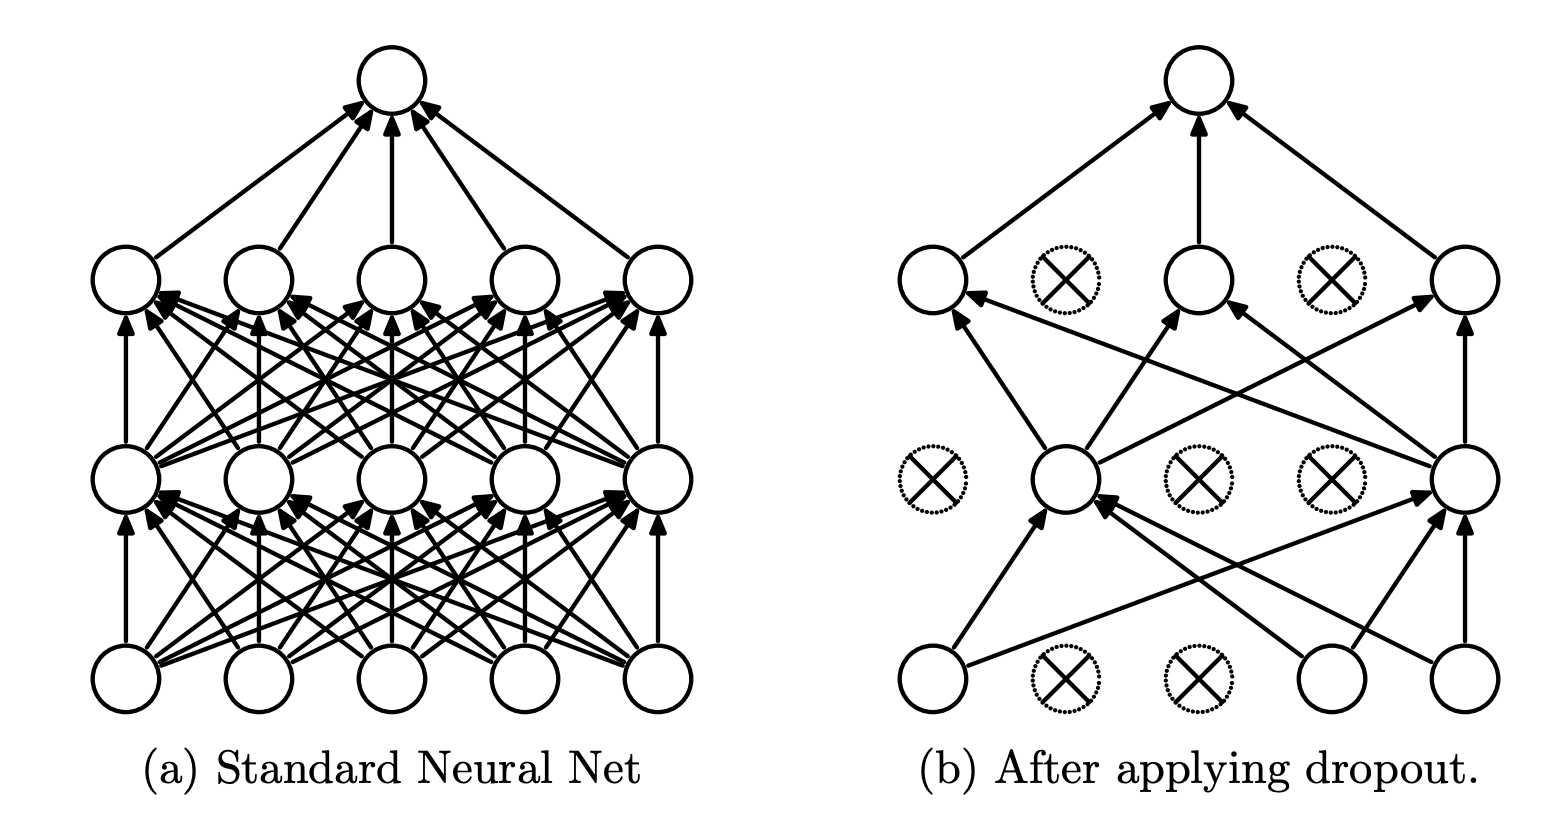
\includegraphics[width=0.8\linewidth]{bilder/dropout.png}
		\caption{Dropout}\label{fig:dropout}
	\end{center}
\end{figure}

From the first training one can clearly see that overfit happens around epoch 30. Although one could just pick out one of epochs before the 30th one (before overfit has happened), applying more regularizion to the model that has been using dropout only would be a good idea. Early stopping in combination with weight decay, BatchNorm were used to regularize the model that was overfitting too quickly with dropout only. $BatchNorm$ layers have been added after the first Convolution layer in each ConvBlock and $TransposedConvBlock$. The results of training the regularized network is presented in Figure \ref{fig:first-train-regularized}.

\begin{figure}[htb]
    \centering
    \begin{minipage}{.5\textwidth}
      \centering
      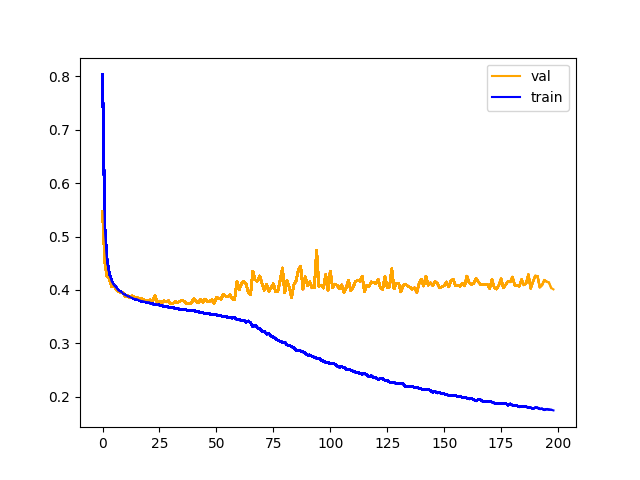
\includegraphics[width=\linewidth]{bilder/firt-train-overfit.png}
      \caption{Not regularized}
      \label{fig:first-train-overfit}
    \end{minipage}%
    \begin{minipage}{.5\textwidth}
      \centering
      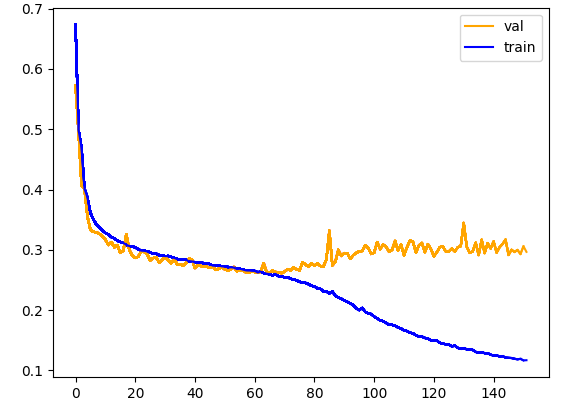
\includegraphics[width=\linewidth]{bilder/first-train-regularized.png}
      \caption{Regularized}
      \label{fig:first-train-regularized}
    \end{minipage}
\end{figure}

\subsubsection{Network reduction}
Since learning a too complex and noise-fitting decision surface might be an often cause of an overfit, another way to mitigate it would to be reduce the space of the possible decision surfaces and therefore make the surface simpler so that it cannot fit into the noise from the data. By changing the number of adaptive parameters in the network, the complexity can be varied. (cite Page 332, Neural Networks for Pattern Recognition, 1995.)

\subsubsection{Expansion of the training data}
To well-tune the hyperparameters the model needs to have a sufficient amount of quality samples. An expanded dataset
can improve the quality of the predictions, (cite doi:10.1088/1742-6596/1168/2/022022) however only when the model has already performed well on the initial dataset. If the model performing bad initially, adding more data will not solve the problem. Here having TODO n samples of data the model was trained on TODO samples only to find the best structure and regularization first, afterwards the model was retrained using more data and the quality imroved from, to TODO.